\documentclass[12pt]{article}
\RequirePackage{amsthm,amsmath,amsbsy,amsfonts}
\usepackage{bm,graphicx,psfrag,epsf}
\usepackage{enumerate}
\usepackage{natbib}
%\RequirePackage[colorlinks,citecolor=blue,urlcolor=blue]{hyperref}
%\RequirePackage{hypernat}
\usepackage{paralist, booktabs, multirow}
%\usepackage{url}


\newtheorem{lemma}{Lemma}
\newcommand{\blind}{0}
\newcommand{\trace}{\text{Trace}}
\numberwithin{equation}{section}
\theoremstyle{plain}
%\newtheorem{thm}{Theorem}[section]
%\newtheorem{mydef}{Definition}
%\newtheorem{remark}{Remark}

%% ----------------------------------------------------------------------
%% Packages
%% ----------------------------------------------------------------------
%\usepackage{amsmath,amsfonts,amssymb}

\usepackage{amssymb}
\usepackage[usenames]{color}
%\usepackage{amsbsy,amsthm,amsmath,amssymb}

%% For \mathscr
\usepackage[mathscr]{eucal}

%% For \llbracket and \rrbracket, \varoast, \varoslash
\usepackage{stmaryrd}

%% For \boldsymbol
%\usepackage{amsbsy}

%%% For \bm (bold math)
%\usepackage{bm}

%% For proper spacing in text macros
\usepackage{xspace}

%% For special lists like inparaenum, compactenum, compactitem
\usepackage{paralist}

%% Turn on/off options for PDF
\usepackage{ifpdf}

%% Graphics
\usepackage{graphicx}
\ifpdf
\usepackage{epstopdf}
% REMOVE NEXT LINE TO REVERT TO PNG FILES
\DeclareGraphicsExtensions{.eps,.pdf}
\else
\usepackage{epsfig}
\fi

%% For \subfloat command
\usepackage{subfig}

%% For hyperlinks. Should always be the last package. Omit for DVI version.
\ifpdf
\usepackage[colorlinks,urlcolor=blue,citecolor=blue,linkcolor=blue]{hyperref}
\else
\newcommand{\href}[2]{{#2}}
\usepackage{url}
\fi

%% For tabulary
\usepackage{tabulary}

%% Show labels
%\usepackage[notref,notcite]{showkeys}

%% Algorithm
\usepackage{algorithm}
\usepackage{algpseudocode}

%% ----------------------------------------------------------------------
%% Hyper-linked References
%% ----------------------------------------------------------------------

\ifpdf
\newcommand{\Sec}[1]{\hyperref[sec:#1]{Section~\ref*{sec:#1}}} %section
\newcommand{\App}[1]{\hyperref[sec:#1]{Appendix~\ref*{sec:#1}}} %appendix
\newcommand{\Eqn}[1]{\hyperref[eq:#1]{{\rm (\ref*{eq:#1})}}} %equation
\newcommand{\Part}[1]{\hyperref[part:#1]{(\ref*{part:#1})}} %part of theorem
\newcommand{\Fig}[1]{\hyperref[fig:#1]{Figure~\ref*{fig:#1}}} %figure
\newcommand{\Tab}[1]{\hyperref[tab:#1]{Table~\ref*{tab:#1}}} %table
\newcommand{\Thm}[1]{\hyperref[thm:#1]{Theorem~\ref*{thm:#1}}} %theorem
\newcommand{\Lem}[1]{\hyperref[lem:#1]{Lemma~\ref*{lem:#1}}} %lemma
\newcommand{\Prop}[1]{\hyperref[prop:#1]{Proposition~\ref*{prop:#1}}} %proposition
\newcommand{\Cor}[1]{\hyperref[cor:#1]{Corollary~\ref*{cor:#1}}} %corollary
\newcommand{\Def}[1]{\hyperref[def:#1]{Definition~\ref*{def:#1}}} %definition
\newcommand{\Alg}[1]{\hyperref[alg:#1]{Algorithm~\ref*{alg:#1}}} %algorithm
\newcommand{\Ex}[1]{\hyperref[ex:#1]{Example~\ref*{ex:#1}}} %example
\newcommand{\As}[1]{\hyperref[as:#1]{Assumption~{\rm\ref*{as:#1}}}} %assumption
\newcommand{\Reg}[1]{\hyperref[as:#1]{Condition~\ref*{reg:#1}}} %regularity condition
\newcommand{\AlgLine}[2]{\hyperref[alg:#1]{line~\ref*{line:#2} of Algorithm~\ref*{alg:#1}}}
\newcommand{\AlgLines}[3]{\hyperref[alg:#1]{lines~\ref*{line:#2}--\ref*{line:#3} of Algorithm~\ref*{alg:#1}}}
\else
\newcommand{\Sec}[1]{{Section~\ref{sec:#1}}} %section
\newcommand{\App}[1]{{Appendix~\ref{sec:#1}}} %appendix
\newcommand{\Eqn}[1]{{(\ref{eq:#1})}} %equation
\newcommand{\Part}[1]{{(\ref{part:#1})}} %part of proof
\newcommand{\Fig}[1]{{Figure~\ref{fig:#1}}} %figure
\newcommand{\Tab}[1]{{Table~\ref{tab:#1}}} %table
\newcommand{\Thm}[1]{{Theorem~\ref{thm:#1}}} %theorem
\newcommand{\Lem}[1]{{Lemma~\ref{lem:#1}}} %lemma
\newcommand{\Prop}[1]{{Property~\ref{prop:#1}}} %property
\newcommand{\Cor}[1]{{Corollary~\ref{cor:#1}}} %corollary
\newcommand{\Def}[1]{{Definition~\ref{def:#1}}} %definition
\newcommand{\Alg}[1]{{Algorithm~\ref{alg:#1}}} %algorithm
\newcommand{\Ex}[1]{{Example~\ref{ex:#1}}} %example
\newcommand{\As}[1]{{Assumption~\ref{as:#1}}} %assumption
\newcommand{\Reg}[1]{{R~\ref{reg:#1}}} %regularity condition
\newcommand{\AlgLine}[2]{{line~\ref{line:#2} of Algorithm~\ref{alg:#1}}}
\newcommand{\AlgLines}[3]{{lines~\ref{line:#2}--\ref{line:#3} of Algorithm~\ref{alg:#1}}}
\fi

\usepackage{paralist, booktabs, multirow}

%% ----------------------------------------------------------------------
%% Environments
%% ----------------------------------------------------------------------

%% Assumptions environments
\newtheorem{assumption}{Assumption}[section]
%% Special proof where box is inside final equation
% The function \proof and \endproof are defined inside the SIAM class file.
% Be sure to use \myproofend inside the final equation to produce the
% special box that signifies the end of the proof.
\newenvironment{myproof}{\proof}{}
\newcommand{\myproofend}{\quad\endproof}
\newtheorem{theorem}{Theorem}[section]


%Added by Arvind
\usepackage[normalem]{ulem}
\newcommand{\arvind}[1]{{\color{red} #1}}


%%%%%

%\RequirePackage[colorlinks,citecolor=blue,urlcolor=blue]{hyperref}
%
%\RequirePackage[OT1]{fontenc}
%\RequirePackage{amsthm,amsmath}
%\RequirePackage [round,authoryear]{natbib}
%\RequirePackage{hypernat}
%
%\usepackage{amsbsy,amsthm,amsmath,amssymb}
%\usepackage{graphicx,booktabs}
%%\usepackage{subfig}
\usepackage{mathtools}
\DeclarePairedDelimiter{\ceil}{\lceil}{\rceil}
\usepackage{algorithm}
\usepackage{algpseudocode}
\usepackage{tikz}
\usetikzlibrary{arrows}
%\setlength{\oddsidemargin}{.75in}
%\setlength{\evensidemargin}{.75in}
%\setlength{\textwidth}{5in}
\newtheorem{proposition}{Proposition}[section]
%\newtheorem{corollary}{Corollary}[section]
%\newtheorem{example}{Example}[section]
%\newtheorem{definition}{Definition}[section]


%% ----------------------------------------------------------------------
%% Definitions
%% ----------------------------------------------------------------------

%% Shorthand for Real
\newcommand{\Real}{\mathbb{R}}
\newcommand{\dom}{{\bf dom}\,}

%% Math notation
\newcommand{\Tra}{^{\sf T}} % Transpose
\newcommand{\Inv}{^{-1}} % Inverse
\newcommand{\tr}{\operatorname{tr}} % Trace
\newcommand{\Ker}{\operatorname{Ker}} % Kernel
\def\vec{\mathop{\rm vec}\nolimits}
\def\mtcz{\mathop{\rm mat}\nolimits} % Matricize operation
\newcommand{\amp}{\mathop{\:\:\,}\nolimits}
\newcommand{\bic}{\text{BIC}}

%% Vectors
\newcommand{\V}[1]{{\bm{\mathbf{\MakeLowercase{#1}}}}} % vector
\newcommand{\VE}[2]{\MakeLowercase{#1}_{#2}} % vector element
\newcommand{\Vbar}[1]{{\bm{\M{A}r \mathbf{\MakeLowercase{#1}}}}} % vector
\newcommand{\Vhat}[1]{{\bm{\hat \mathbf{\MakeLowercase{#1}}}}} % vector
\newcommand{\Vtilde}[1]{{\bm{\tilde \mathbf{\MakeLowercase{#1}}}}} % vector
\newcommand{\Vn}[2]{\V{#1}^{(#2)}} % n-th vector
\newcommand{\VnE}[3]{{#1}^{(#2)}_{#3}} % n-th vector
\newcommand{\VtildeE}[2]{\tilde{\MakeLowercase{#1}}_{#2}} % vector element


%% Matrices
\newcommand{\M}[1]{{\bm{\mathbf{\MakeUppercase{#1}}}}} % matrix
\newcommand{\ME}[2]{\MakeLowercase{#1}_{#2}} % matrix element
\newcommand{\MC}[2]{\V{#1}_{#2}}
\newcommand{\Mr}[2]{\V{#1}_{#2}} % matrix row
\newcommand{\Mhat}[1]{{\bm{\hat \mathbf{\MakeUppercase{#1}}}}} % matrix
\newcommand{\Mtilde}[1]{{\bm{\tilde \mathbf{\MakeUppercase{#1}}}}} % matrix
\newcommand{\MhatC}[2]{\Vhat{#1}_{#2}} % matrix column
\newcommand{\Mbar}[1]{{\bm{\M{A}r \mathbf{\MakeUppercase{#1}}}}} % matrix
\newcommand{\MbarC}[2]{\Vbar{#1}_{#2}} % matrix column
\newcommand{\Mn}[2]{\M{#1}^{(#2)}} % n-th matrix
\newcommand{\Mbarn}[2]{\Mbar{#1}^{(#2)}} % n-th matrix
\newcommand{\Mtilden}[2]{\Mtilde{#1}^{(#2)}} % n-th matrix
\newcommand{\MnTra}[2]{\M{#1}^{(#2){{\sf T}}}} % n-th matrix transpose
\newcommand{\MnE}[3]{\MakeLowercase{#1}^{(#2)}_{#3}} % n-th matrix element
\newcommand{\MnC}[3]{\V{#1}^{(#2)}_{#3}} % n-th matrix column
\newcommand{\MbarnC}[3]{\Vbar{#1}^{(#2)}_{#3}} % n-th matrix column
\newcommand{\MnCTra}[3]{\V{#1}^{(#2){{\sf T}}}_{#3}} % n-th matrix column transpose
\newcommand{\MCTra}[2]{\V{#1}^{{\sf T}}_{#2}} % n-th matrix column transpose

%% Tensors
\newcommand{\T}[1]{\boldsymbol{\mathscr{\MakeUppercase{#1}}}} %tensor
\newcommand{\Tbar}[1]{\boldsymbol{\M{A}r \mathscr{\MakeUppercase{#1}}}} %tensor
\newcommand{\That}[1]{\boldsymbol{\hat \mathscr{\MakeUppercase{#1}}}} %tensor
\newcommand{\Ttilde}[1]{\boldsymbol{\tilde \mathscr{\MakeUppercase{#1}}}} %tensor
\newcommand{\TE}[2]{\MakeLowercase{#1}_{\MI{#2}}} % tensor element with multi-index

%% Matrix-matrix operations
\newcommand{\Kron}{\otimes} %Kronecker
\newcommand{\Khat}{\odot} %Khatri-Rao
\newcommand{\Hada}{\ast} %Hadamard
\newcommand{\Divide}{\varoslash}

% Matricize
\newcommand{\Mz}[2]{\M{#1}_{(#2)}} % n-th mode matricize
\newcommand{\Mzsets}[3]{\TM{#1}{#2\times#3}} % matricze with just the sets specified
\newcommand{\Mzall}[4]{\TM{#1}{#2\times#3\,:\,#4}} % full matricize specification

%% K-Tensor
\newcommand{\KT}[1]{\left\llbracket #1 \right\rrbracket} % kruskal operator
\newcommand{\KTsmall}[1]{\llbracket #1 \rrbracket} % small kruskal operator
\newcommand{\KG}[1]{\langle #1 \rangle} % kruskal "group"

%% text with quads around it
\newcommand{\qtext}[1]{\quad\text{#1}\quad}

%% Derivative
\newcommand{\FD}[2]{\frac{\partial #1}{\partial #2}}

%% Prox-operator
\newcommand{\prox}[2]{\operatorname{prox}_{#1}({#2})}

%% Sign-operator
\newcommand{\sign}[1]{\operatorname{sign}({#1})}

%% convex hull
\newcommand{\conv}[1]{\operatorname{conv}({#1})}

%% For comments to each other
\newcommand{\Remark}[2]{{\color{red}Remark from #1: #2}\xspace}
\newcommand{\Note}[1]{{{\color{red}{#1}}}\xspace}

%\startlocaldefs
%\numberwithin{equation}{section}
%\theoremstyle{plain}
%\newtheorem{thm}{Theorem}[section]
%\endlocaldefs

\addtolength{\oddsidemargin}{-.5in}%
\addtolength{\evensidemargin}{-.5in}%
\addtolength{\textwidth}{1in}%
\addtolength{\textheight}{1.3in}%
\addtolength{\topmargin}{-.8in}%

\pdfminorversion=4

%% ----------------------------------------------------------------------
%% Main Document
%% ----------------------------------------------------------------------
\begin{document}

\def\spacingset#1{\renewcommand{\baselinestretch}%
{#1}\small\normalsize} \spacingset{1}


%%%%%%%%%%%%%%%%%%%%%%%%%%%%%%%%%%%%%%%%%%%%%%%%%%%%%%%%%%%%%%%%%%%%%%%%%%%%%%

\if0\blind
{
  \title{\bf Drift Removal for Time Series Data Using Quantile Trend Filtering}
  \author{Halley Brantley\thanks{
    Department of Statistics, North Carolina State University, Raleigh, NC 27695-8203 (E-mail: hlbrantl@ncsu.edu)} \,
         Joseph Guinness\thanks{
    Department of Statistics, North Carolina State University, Raleigh, NC 27695-8203 (E-mail: jsguinne@ncsu.edu)} \,
    and
%    and
    Eric C. Chi\thanks{Department of Statistics, North Carolina State University, Raleigh, NC 27695-8203 (E-mail: eric$\_$chi@ncsu.edu).}    \\}
    \date{}
  \maketitle
} \fi

\if1\blind
{
  \bigskip
  \bigskip
  \bigskip
  \begin{center}
    {\LARGE\bf Title}
\end{center}
  \medskip
} \fi

\bigskip
\begin{abstract}
Abstract
\end{abstract}

\noindent%
{\it Keywords:}  Key words
\vfill

\newpage
\spacingset{1.45} % DON'T change the spacing!
%% ----------------------------------------------------------------------
%% Introduction
%% ----------------------------------------------------------------------
\section{Introduction}

\subsection{Background}

\begin{itemize}
\item \cite{Oh2011} unified framework for non-parametric quantile regression by approximating check loss function with quadratic loss near zero.
\item \cite{KoenkerNgPortnoy1994} introduce quantile smoothing splines. We need to discuss how our approach is different.
\item \cite{Kim2009} introduce the concept of $\ell_1$-trend filtering.
\item \cite{Tib2014} describes properties of trend filtering using quadratic loss. Shows that trend filtering estimates adapt to the local level of smoothness much better than smoothing splines, and exhibit a remarkable similarity to locally adaptive regression splines. Prove that (with the right choice of tuning parameter) the trend filtering estimate
converges to the true underlying function at the minimax rate for functions whose kth derivative is of bounded variation.
\item \cite{Ning2014} address problem of estimating a smooth baseline in noisy data with drift.
\item \cite{Takeuchi2006nonparametric} Nonparametric quantile regression using SVM with Gaussian RBF kernels and check (pinball) loss. 
\item \cite{yuan2006gacv} Comparison of cross-validation methods for quantile smoothing splines.  
\end{itemize}
We propose to use the trend filtering penalty with the check loss function to produce a non-parametric quantile regression estimate that can be computes using a linear time algorithm for removing trends in time series. The formulation was proposed by \cite{Kim2009} as a possible extension of $\ell_1$-trend filtering but not studied. Moreover we extend the basic framework to model multiple quantiles and ensure non-crossing. 

\subsection{Application}

	 \begin{figure}[!h] 
	 	\caption{Raw Data - three collocated sensors}
		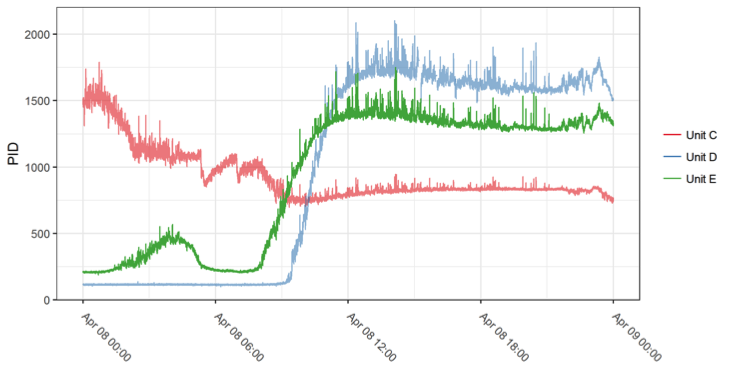
\includegraphics[width = 5in]{Figures/spodRaw.png}
	\end{figure}
	 \begin{figure}[!h] 
	 	\caption{Detrended data - three collocated sensors}
	\includegraphics[width = 5in]{Figures/spodDetrended.png}
	\end{figure}

Examples:
\begin{itemize}
\item Air quality \citep{Apte2017}
\item ECG \citep{Sanyal2012}
\item Chromatogram baseline estimation  \citep{Ning2014, Ilewicz2015}
\item Galaxy spectrum baseline estimation \citep{Ilewicz2015,Bacher2016}
\item Identifying absorption dips from black body radiation
\end{itemize}

Need to decide between detrending versus detrending + denoising. The BEADS \citep{Ning2014} method does both. We may wish to focus on detrending and then use wavelet SURE denoising as a postprocessing step, i.e. do a two-stage procedure, both of which can be done in linear time. On paper this should be faster than the BEADS procedure. Or we may just want to stick with detrending.  There's Matlab code for BEADS, and the BEADS paper also points to two other popular methods in chromotography. 

Things to do:
\begin{itemize}
	\item Convergence of the algorithm
	\item Convergence rate \citep{He2012, He2015, Davis2017}
	\item Timing experiments of LP versus Spingarn
	\item Make an R package - detrendr
	\item Compare on synthetic data quality of solution with existing methods
	\item Do comparisons on real data examples
\end{itemize}

%% ----------------------------------------------------------------------
%% Quantile Regression
%% ----------------------------------------------------------------------
\section{Quantile Regression}

The classic least squares regression is notoriously sensitive to outliers. One remedy to blunt the influence of outliers is to compute the least absolute deviations (LAD) solution in place of the least squares one. Given a design matrix $\M{X} \in \Real^{n \times p}$ and continuous responses $\V{y} \in \Real^n$, we estimate a regression vector $\V{\theta} \in \Real^p$ so that $\M{X}\V{\theta}$ is a good approximation of $\V{y}$. The LAD estimator is a solution to the problem
\begin{eqnarray*}
\underset{\V{\theta}}{\min}\; \frac{1}{n}\lVert \V{y} - \M{X}\V{\theta} \rVert_1.
\end{eqnarray*}
The above optimization problem generalizes the notion of the median of a collection of numbers. A median $\mu$ of $n$ reals $\VE{y}{1}, \ldots, \VE{y}{n}$ is the minimizer of the function
\begin{eqnarray*}
f(u) & = & \frac{1}{n}\sum_{i=1}^n \lvert \VE{y}{i} - \theta \rvert.
\end{eqnarray*}
Recall that the median is the 50th percentile or 0.5-quantile, namely half of the $\VE{y}{i}$ are less than or equal to $\mu$ and the other half is greater than or equal to $\mu$. The median can be generalized to arbitrary $\tau$-quantiles for $\tau \in (0,1)$ to give us quantile regression \citep{Koenker1978}.

First define the so-called ``check function"
\begin{eqnarray*}
\rho_\tau(\Delta) & = & \begin{cases}
\tau \Delta & \text{$\Delta \geq 0$} \\
-(1-\tau)\Delta & \text{$\Delta < 0$}. \\
\end{cases}
\end{eqnarray*}
Then the $\tau$th quantile of the $\VE{y}{i}$ is a minimizer of the function
\begin{eqnarray*}
f_\tau(\theta) & = & \frac{1}{n}\sum_{i=1}^n \rho_\tau(\VE{y}{i} - \theta).
\end{eqnarray*}
Returning to the regression context, we can generalize LAD regression to quantile regression, namely computing the minimizer of the function
\begin{eqnarray*}
f_\tau(\V{\theta}) & = & \frac{1}{n}\sum_{i=1}^n \rho_\tau(\VE{y}{i} - \langle \V{x}_i \mid \V{\theta} \rangle),
\end{eqnarray*}
where $\V{x}_i \in \Real^p$ denotes the $i$th row of $\M{X}$.

%% ----------------------------------------------------------------------
%% Trend Filtering
%% ----------------------------------------------------------------------
\section{Trend Filtering}

In the trend filtering problem \citep{Kim2009, Tib2014}, one is interested in finding an adaptive polynomial approximation to noisy data $\V{y} \in \Real^n$ by solving the following convex problem.
\begin{eqnarray*}
\underset{\V{\theta}}{\arg\min}\; \frac{1}{2n} \lVert \V{y} - \V{\theta} \rVert_2^2 + \lambda \lVert \Mn{D}{k+1}\V{\theta} \rVert_1,
\end{eqnarray*}
where $\lambda \geq 0$ is a regularization parameter that trades off the emphasis on the data fidelity term and the matrix $\Mn{D}{k+1} \in \Real^{(n - k -1) \times n}$ is the discrete difference operator of order $k+1$. To understand the purpose of penalizing $\Mn{D}{k+1}$ consider the difference operator when $k = 0$.
\begin{eqnarray*}
\Mn{D}{1} = \begin{pmatrix}
-1 & 1 & 0 & \cdots & 0 & 0 \\
0 & -1 & 1 & \cdots & 0 & 0 \\
\vdots & & & & & \\
0 & 0 & 0 & \cdots & -1 & 1 \\
\end{pmatrix}
\end{eqnarray*}
Thus, $\lVert \Mn{D}{1}\V{\theta} \rVert_1 = \sum_{i=1}^{n-1} \lvert \VE{\theta}{i} - \VE{\theta}{i+1} \rvert$ which is just total variation denoising in one dimension. The penalty incentivizes solutions which are piece-wise constant. For $k \geq 1$, the difference operator $\Mn{D}{k+1} \in \Real^{(n-k-1) \times n}$ is defined recursively as follows
\begin{eqnarray*}
\Mn{D}{k+1} & = & \Mn{D}{1}\Mn{D}{k}.
\end{eqnarray*}
By penalizing the $k+1$ fold composition of the discrete difference operator, we obtain solutions which are piecewise polynomials of order $k$.

%% ----------------------------------------------------------------------
%% Quantile Trend Filtering
%% ----------------------------------------------------------------------
\section{Quantile Trend Filtering}

We combine the ideas of quantile regression and trend filtering, namely consider the signal approximation problem, where the design $\M{X}$ is the identity matrix.

The estimation of the quantile trend filtering model can be posed as the following optimization problem.
\begin{eqnarray}
\label{eq:quantile_trend}
	\underset{\V{\theta}}{\min}\; \frac{1}{n} \sum_{i=1}^n \rho_\tau(\VE{y}{i} - \VE{\theta}{i}) + \lambda \lVert \Mn{D}{k} \V{\theta} \rVert_1,
\end{eqnarray}
where $\lambda$ is a nonnegative tuning parameter. As with the classic quantile regression, the quantile trend filtering problem can be solved by a linear program. We argue that it is better solved by Spingarn's method of partial inverses.


\section{Related Work}

\begin{itemize}
	\item Quantile splines \citep{Oh2011}
	\item BEADS 
\end{itemize}

%% ----------------------------------------------------------------------
%% Spingarn's method of partial inverses
%% ----------------------------------------------------------------------
\section{Spingarn's method of partial inverses}

We first review Spingarn's method \citep{Spingarn1985}, which solves the following equality constrained convex problem:
\begin{equation}
\label{eq:spingarn}
\begin{split}
\text{minimize}\; & \psi(\V{x}) \\
\text{subject to}\; & \V{x} \in V,
\end{split}
\end{equation}
where $V$ is a subspace. The problem \Eqn{spingarn} can be expressed as the unconstrained optimization problem
\begin{equation}
\label{eq:spingarn2}
\text{minimize}\; \psi(\V{x}) + \iota_V(\V{x}),
\end{equation}
where $\iota_V$ is the indicator function of the set $V$. Spingarn's method applies Douglas-Rachford splitting to the problem \Eqn{spingarn2} to give the following updates.

\begin{eqnarray*}
\Vn{x}{k+1} & = & \prox{t\psi}{\Vn{z}{k}} \\
\Vn{y}{k+1} & = & P_V\left(2\Vn{x}{k+1} - \Vn{z}{k} \right) \\
\Vn{z}{k+1} & = & \Vn{z}{k} + \lambda^{(k)}\left(\Vn{y}{k+1} - \Vn{x}{k+1} \right).
\end{eqnarray*}
The parameter $t$ is a step-size and $\lambda^{(k)}$ is Krasnosel'ski{\u i}-Mann iteration (Need citation). We require that $\lambda^{(k)} \in ]0, 2[$ and that $\sum_n \lambda^{(k)} (2-\lambda^{(k)}) = \infty$. The mapping $P_V$ is the orthogonal projection onto the set $V$.  Note that the algorithm iterates $\Vn{x}{k}$ will converge to a solution to problem $\Eqn{spingarn}$ \citep{Combettes2005}. We need to experiment with different over / under-relaxation parameters $\lambda^{(k)}$ and step sizes $t$. It will converge if we take $\lambda^{(k)} = 1$ and $t = 1$, but we may be able to converge faster in practice by taking non-trivial values.

%% ----------------------------------------------------------------------
%% Applying Spingarn's Method to Quantile Trend Filtering
%% ----------------------------------------------------------------------
\section{Applying Spingarn's Method to Quantile Trend Filtering}

To simplify the notation we suppress the order $k$ and write $\Mn{D}{k}$ as $\M{D}$.
We can reformulate our optimization problem \Eqn{quantile_trend} as the following equality constrained convex optimization problem.

\begin{eqnarray*}
\text{minimize}\; && f_1(\V{\theta}) + f_2(\V{\eta}) \\
\text{subject to}\; && \V{\eta} = \M{D}\V{\theta}
\end{eqnarray*}
where
\begin{eqnarray*}
f_1(\V{\theta}) = \frac{1}{n}\sum_{i=1}^n \rho_\tau(\VE{y}{i} - \VE{\theta}{i}) \quad\quad \text{and} \quad\quad
f_2(\V{\eta}) = \lambda\lVert \V{\eta} \rVert_1.
\end{eqnarray*}

If we set $\psi(\V{\theta}, \V{\eta}) = f_1(\V{\theta}) + f_2(\V{\eta})$ and $V = \{ \V{z}\Tra = (\V{\theta}\Tra, \V{\eta}\Tra) : \V{\eta} = \M{D}\V{\theta} \}$, then we can apply Spingarn's method. Note that
\begin{eqnarray*}
\prox{th}{\V{\theta}, \V{\eta}} & = & (\prox{tf_1}{\V{\theta}}, \prox{tf_2}{\V{\eta}}) \\
P_V(\V{\theta}, \V{\eta}) & = & \begin{pmatrix}
\M{I} \\ \M{D}
\end{pmatrix}
\begin{pmatrix}
\M{I} + \M{D}\Tra\M{D}
\end{pmatrix}\Inv
\begin{pmatrix}
\V{\theta} + \M{D}\Tra\V{\eta}
\end{pmatrix},
\end{eqnarray*}
where the projection $P_V$ requires a banded linear system solve, with bandwidth $k + 1$.
This linear solve can be accomplished in $\mathcal{O}(n(k + 1)^2)$. The first solve using a banded Cholesky decomposition requires $\mathcal{O}(n(k + 1)^2)$. Subsequent solves require
$\mathcal{O}(n(k+1))$. We can use RccpArmadillo to do banded Cholesky \citep{Eddelbuettel2014}.

%% ----------------------------------------------------------------------
%% Proximal mappings
%% ----------------------------------------------------------------------
\subsection*{Proximal mappings}

We need the proximal mappings for $tf_1$ and $tf_2$.

\begin{eqnarray*}
\left [\prox{tf_1}{\V{\theta}} \right ]_i & = & \VE{y}{i} - \prox{(t/n)\rho_\tau}{\VE{y}{i} - \VE{\theta}{i}}, \\
\left [\prox{tf_2}{\V{\eta}} \right ]_j & = & S(\VE{\eta}{j}, t\lambda).
\end{eqnarray*}

The proximal mapping for $tf_2$ is the element-wise softhresholding operator. We now derive the  proximal mapping of $\rho_\tau(\Delta)$, which can be evaluated in closed form. We need to find the minimizer of the following univariate function
\begin{eqnarray*}
g_\tau(\Delta) & = & \Delta[\tau - I(\Delta < 0)] +  \frac{n}{2t} (\Delta - w)^2, \\
\end{eqnarray*}
where $w \in \Real$ is given and $I(\Delta < 0)$ is 0 when $\Delta < 0$ and 1 otherwise.

The subgradient of $\rho_\tau(\Delta) = \Delta[\tau - I(\Delta < 0)]$ is given by
\begin{eqnarray*}
\partial \rho_\tau(\Delta) & = & \begin{cases}
\tau & \text{if $\Delta > 0$} \\
\tau - 1 & \text{if $\Delta < 0$} \\
[\tau - 1, \tau] & \text{if $\Delta = 0$}.
\end{cases}
\end{eqnarray*}
The stationary condition is
\begin{eqnarray*}
\frac{n}{t}[w - \Delta] & \in & \partial \rho_\tau(\Delta).
\end{eqnarray*}
Therefore, the proximal mapping is given by 
\begin{eqnarray*}
\prox{(t/n) \rho_\tau}{w} & = & \begin{cases}
w - \tau \frac{t}{n}& \text{if $w > \tau \frac{t}{n}$} \\
w + (1-\tau)\frac{t}{n} & \text{if $w < - (1-\tau)\frac{t}{n}$} \\
0 & \text{if $-(1- \tau)\frac{t}{n} \leq w \leq \tau \frac{t}{n}$.}
\end{cases}
\end{eqnarray*}




\subsection*{Computational Costs}

\subsubsection*{Precomputation}

The following calculations need only be done once. 

\begin{itemize}
\item $\mathcal{O}(n(k + 1)^2)$ to compute the banded Cholesky factorization of $\M{I} + [\Mn{D}{k}]\Tra[\Mn{D}{k}]$
\end{itemize}

\subsubsection*{Per-Iteration}

The following calculations will be done every iteration.

\begin{itemize}
\item $\mathcal{O}(n)$ to compute $\prox{t\psi}{\V{\theta}, \V{\eta}}$
\item $\mathcal{O}((k+1)(n-k+1))$ to compute $\V{\theta} + [\Mn{D}{k}]\Tra\V{\eta}$
\item $\mathcal{O}(n(k+1))$ to compute $\V{\phi} = (\M{I} +[\Mn{D}{k}]\Tra[\Mn{D}{k}] )\Inv(\V{\theta} + \M{D}\Tra\V{\eta})$
\item $\mathcal{O}((k+1)(n-k+1))$ to compute $\begin{pmatrix}
\M{I} \\ \Mn{D}{k} \end{pmatrix}\V{\phi}$
\end{itemize}

The total cost is $\mathcal{O}(nk)$.

\subsection{Summary}

\begin{itemize}
\item The overall computational complexity is essentially linear $\mathcal{O}(nk^2)$ for the initial banded Cholesky decomposition and the per-iteration complexity is $\mathcal{O}(nk)$.
\item One could also apply Anderson acceleration \citep{Walker2011} to reduce the number of Spingarn updates, since the Douglas-Rachford algorithm is a fixed point algorithm.
\end{itemize}

%% ----------------------------------------------------------------------
%% Applying Spingarn's Method to Quantile Trend Filtering version 2
%% ----------------------------------------------------------------------
\section{Applying Spingarn's Method to Quantile Trend Filtering version 2}

Following the specialized ADMM algorithm for trend filtering \citep{Ramdas2016}, we can also take advantage of fast exact solvers of the one-dimensional fussed lasso problem \citep{davies2001, Johnson2013}. The first method is based on taut strings, and the second is based on dynamic programming. Both of these methods run in linear time. A third exact method with worst case quadratic penalty but linear time in typical cases was proposed by \cite{Condat2013}. C code is available for all three methods. We should compare them.

What is the reparameterization?

\begin{eqnarray*}
\text{minimize}\; && f_1(\V{\theta}) + f_2(\V{\eta}) \\
\text{subject to}\; && \V{\eta} = \M{D}\V{\theta}
\end{eqnarray*}
where
\begin{eqnarray*}
f_1(\V{\theta}) = \frac{1}{n}\sum_{i=1}^n \rho_\tau(\VE{y}{i} - \VE{\theta}{i}) \quad\quad \text{and} \quad\quad
f_2(\V{\eta}) = \lambda\lVert \Mn{D}{1}\V{\eta} \rVert_1.
\end{eqnarray*}

Difference with version 1: If we are interested in a 3rd order penalization, then $\M{D} = \Mn{D}{2}$ in version 2 as opposed to $\M{D} = \Mn{D}{3}$ in version 1. The proximal mapping for $f_2$ is solved using one of the exact solvers \citep{davies2001, Johnson2013, Condat2013}. Show some timing results between the different versions. Point readers to \cite{Ramdas2016} for a discussion of why this minor reparameterization may lead to speed up.

\section{Other Practical Issues}

\begin{itemize}
	\item Read compressed data
	\item May want to read data directly in C and not pull into R; make R just an interface
	\item Use historical data to choose $\tau$ and $\lambda$
\end{itemize}

\section{To Do}

\begin{itemize}
	\item Find out if we can use the EPA data. Add co-authors?
	\item Make version 2 with the three fast fused lasso solvers
	\item Add homotopy / warm start
	\item Add model selection
	\item Do experiments to evaluate different choices of $t$ and $\lambda^{(k)}$
	\item See if Anderson acceleration helps. Talk to Tim Kelley?
	\item Write vignette
	\item Do comparisons with BEAD
	\item Do wind polar plots with and without removing trends
	\item Compare with Splines
\end{itemize}

\section{Numerical Studies}

We compare our detrending method with BEADS and the more general nonparametric quantile method introduced by \cite{Oh2011}.

\bibliographystyle{asa}
\bibliography{detrendify}

\end{document}  

